\chapter{Force-Guided Robot Alignment}
This chapter follows on from the previous chapter, we continue to demonstrate some technical solutions of system integration. On top of that, Forces and Torques (F/T) sensor will be included to discuss. Therefore, you can see the chapter as a operating manual when you simultaneously own a robot arm, an F/T sensor and an end effector. First of all, we explain why we will use F/T sensor in our project in section \ref{sec:pro def}. Furthermore, we introduce how to do gravity compensation in senction \ref{sec:grav compen}. Admittance control based on F/T sensor is described in section \ref{sec:adm ctrl}. Reference Frame Changing of F/T sensor is interpreted in section \ref{sec:rfc}. Last but not least, we discuss affection of setting admittance control parameters in section \ref{sec:affection}.
\section{Problem Definition}
\label{sec:pro def}
(Main cause of surgical failure)
(Peg in hole method based on F/T feedback)
(Modes: Doctor Dragging and self-alignment)
how to compensate the gravity affection in section \ref{sec:grav compen}; how to use admittance control in section with F/T sensor \ref{sec:adm ctrl}; and how to obtain the real force and torque values in the tool tip frame in section \ref{sec:rfc}
\section{Integration of F/T sensor}
\label{sec:grav compen}
Gravity compensation is a standard technical issue when combining an F/T sensor, a robot arm and an end effector.
\section{Alignment to the Root Canal (Dragging for alignment)}
In the hope that dentist could drag our system to the infected teeth by holding the end effector, we usher in admittance control based on F/T sensor.
\subsection{Admittance Control based on F/T sensor}
Admittance control make the robot move like a spring-mass-damper system. Forces and torques can be mapped into the movements such as position or velocity. Most important of all, admittance control enables an robot arm to cooperate with human in a safe work environment.Since Meca500 is an industrial robot arm without admittance control, we subsequently combine the robot arm with the F/T sensor so as to adopt admittance control. With force and torque feedback, F/T sensor make Meca500 be resemble to a collaborative robot arm. Therefore, we propose a control scheme depicted as Figure \ref{fig:adm ctrl}. It's worth noting that in this approach the admittance control function is triggered by the end effector mounted on F/T sensor instead of detecting each wrist torque of the robot arm.

\label{sec:adm ctrl}
\begin{figure}[htbp]
\begin{center}
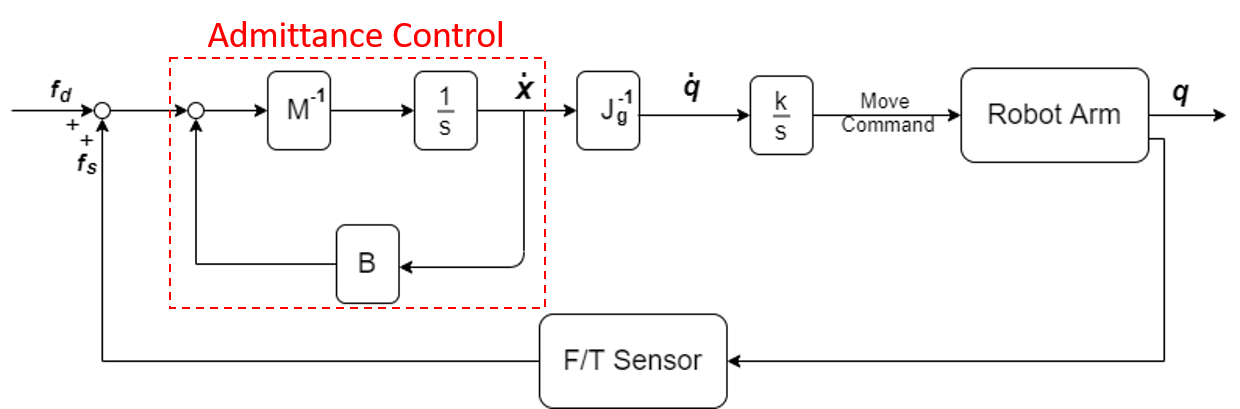
\includegraphics[width=1\linewidth]{Images/adm ctrl.png}
\end{center}
\caption{
Control scheme. $\boldsymbol{f_d}$ denotes the desired forces and torques vector. $\boldsymbol{f_s}$ denotes the real value detected by F/T sensor and is also a forces and torques vector. $\boldsymbol{\dot{x}}$ denotes [$\dot{x}, \dot{y}, \dot{z}, \dot{\theta _x}, \dot{\theta _y}, \dot{\theta _z}$]. $\mathbf{J_g}$ denotes the geometric Jacobian matrix. $\boldsymbol{\dot{q}}$ denotes [$\dot{\theta _1}, \dot{\theta _2}, \dot{\theta _3}, \dot{\theta _4}, \dot{\theta _5}, \dot{\theta _6}$]. $\boldsymbol{q}$ denotes $\left[\theta _1, \theta _2, \theta _3, \theta _4, \theta _5, \theta _6 \right] $.
}\label{fig:adm ctrl}
\end{figure}

A standard equation of admittance control is represented as Equation \ref{eq:adm_mbk}. The values we obtain from the F/T sensor are $\left[f_x, f_y, f_z,\tau _x, \tau _y, \tau _z \right]$, whose forces $ \left[f_x, f_y, f_z\right]$ are related to the translations $ \left[x, y, z\right]$ and torques $ \left[\tau _x, \tau _y, \tau _z\right]$ are related to the axis angle $ \left[\theta _x,\theta _y,\theta _z\right]$. 
\begin{equation}
\label{eq:adm_mbk}
\begin{split}
\begin{bmatrix}
x \\
y \\
z \\
\theta _x \\
\theta _y \\
\theta _z 
\end{bmatrix}
=
\frac{1}{\mathbf{M}\mathrm{S}^2+\mathbf{B}\mathrm{S}+\mathbf{K}}
\begin{bmatrix}
f_x \\
f_y \\
f_z \\
\tau _x \\
\tau _y \\
\tau _z 
\end{bmatrix}
\end{split}
\end{equation}
In our proposed approach we omit parameter $\mathbf{K}$ which is relevant to spring stiffness, considering that it's not necessary to bounce such as a spring. Therefore, our system should behave like a mass-damper system as following.
\begin{equation}
\label{eq:adm_mb}
\begin{split}
\begin{bmatrix}
x \\
y \\
z \\
\theta _x \\
\theta _y \\
\theta _z 
\end{bmatrix}
=
\frac{1}{\mathbf{M}\mathrm{S}^2+\mathbf{B}\mathrm{S}}
\begin{bmatrix}
f_x \\
f_y \\
f_z \\
\tau _x \\
\tau _y \\
\tau _z 
\end{bmatrix}
\end{split}
\end{equation}
where $\mathbf{M},\mathbf{B},\mathbf{K}$ are diagonal positive definite matrices. Affections of these parameters will be discussed in section \ref{sec:affection}.

After determining our admittance control model, we should select a correspondent command to move the robot. However there are many commands of moving the robot arm such as position command - MoveJoints $\left(\theta _1, \theta _2,\cdots , \theta _6 \right)$ and MovePose $\left(x,y,z,\alpha ,\beta ,\gamma \right)$; velocity command - MoveJointsVel $\left(\dot{\theta}_1, \dot{\theta}_2,\cdots , \dot{\theta}_6 \right)$ and MoveLinVelTRF $\left(\dot{x},\dot{y},\dot{z},\dot{\theta _x},\dot{\theta _y},\dot{\theta _z}\right)$. Considering the singularity problem is an imperative problem in robotics, we intend to use MoveJoints or MoveJointsVel to directly set the angles of axis. Despite that it's easier to implement admittance control via other commands, the system would touch the singularity point at any time. It undoubtedly expose patients to danger because the uncertainty of the system. Therefore, position command - MoveJoints and velocity command - MoveJointsVel is our options. Why we choose the command MoveJoints  is that Meca500 has a default time-out value to essure its safty. Despite we could set this value from 0.001 to 2 second, Meca500 is still restricted to move with this value. For example, the value of time-out is set $0.1$ sec. While the robot receive a command, the robot move for $0.1$ sec then immideatly stop. It's not easy to control via velocity command due to this default property.

Finally, we designate MoveJointsVel $\left(\dot{\theta}_1, \dot{\theta}_2,\cdots , \dot{\theta}_6 \right)$ as our main command. Thanks to the property of Jacobian matrix shown in Equation \ref{eq:jg6}, we can transform $\boldsymbol{\dot{x}}$ into $\boldsymbol{\dot{q}}$. Then we multiply it an integrator $\frac{1}{\mathrm{S}}$
to obtain $\boldsymbol{q}$. Note that, As F/T sensor is mounted on the frame\{6\}, we should use Equation \ref{eq:jg6} rather than Equation \ref{eq:jg0}. 
\section{Alignment to the Root Canal (Drilling and self-alignment)}
\subsection{Reference Frame Changing of F/T sensor}
\label{sec:rfc}
(Transformation from robot to tool [Chapt. 3.4]+ Transformation from sensor to tool) 
(How to find the direction vector of the tool)
(From sensor frame to tool tip frame)
\subsection{Motion Planning: Based on Admittance Control}
(Block diagram, robot command choice)
\section{Discussion about Affection of Parameter Setting}
\label{sec:affection}
(K, Bi, Mi- without numbers)
(Modes: Doctor Dragging and Self-alignment - with numbers; get reasonable and suitable parameters first)